\appendix
\section{Appendix of proofs}
\subsection{\texorpdfstring{$\lambda$}{{}} is the smallest singular value of \texorpdfstring{$\hat{X}$}{{}}}\label{appendix:smallest_singular_value}
\noindent For that we need to follow what \cite{THOMPSON19721} has stated in theorem 1 and apply it to our case, therefore: let $\hat{X}$ be an $m\times n$ matrix where $\hat{X}=\begin{bmatrix}
    X^T\\
    \lambda I
\end{bmatrix}$ with $X^T \in \mathbb{R}^{k\times n}$, whose singular values are $\sigma_1(\hat{X})\geq \dots \geq \sigma_n(\hat{X})$. Let $\lambda I$ be a $n\times n$ submatrix of $\hat{X}$, with singular values $\sigma_1(\lambda I)\geq \dots \geq \sigma_n(\lambda I)$, then
\begin{subequations}
    \begin{equation}
        \label{eq:proof_singular_value_1}
        \sigma_i(\hat{X}) \geq \sigma_i(\lambda I), \hspace{3mm }for \hspace{3mm} i=1,\dots, n
    \end{equation}
    \begin{equation}
        \label{eq:proof_singular_value_2}
        \sigma_i(\lambda I) \geq \sigma_{i+k}(\hat{X}), \hspace{3mm }for \hspace{3mm} i\leq min(n-k, n)
    \end{equation}
    with $k=m-n$.
\label{eq:proof_singular_value}
\end{subequations}
\vspace{3mm}

\noindent Let's consider the $(n-k)th$ singular value of $\lambda I$, following \eqref{eq:proof_singular_value_2} we have that
\begin{equation}
    \sigma_n(\hat{X}) \leq \sigma_{n-k}(\lambda I)
    \label{eq:proof_singular_value_3}
\end{equation}
Then by putting \eqref{eq:proof_singular_value_1} into \eqref{eq:proof_singular_value_3} we obtain
\begin{equation}
    \sigma_n(\lambda I) \leq \sigma_n(\hat{X}) \leq \sigma_{n-k}(\lambda I)
    \label{eq:proof_singular_value_4}
\end{equation}
$\lambda I$ is an $n\times n$ matrix whose singular values are all equal to $\lambda$, therefore from \eqref{eq:proof_singular_value_4} we can easily state that
\begin{equation}
    \sigma_n(\hat{X})=\lambda
    \label{eq:least_singular_value}
\end{equation}

\subsection{Condition number of \texorpdfstring{$\hat{X}$}{{}}}\label{appendix:condition_number}
As we know from the theory, the condition number $\kappa$ of a matrix is the following
\begin{equation}
    \kappa(\hat{X}) = \frac{\sigma_1}{\sigma_n}
    \label{eq:condition_number}
\end{equation}
where $\sigma_1$ and $\sigma_n$ are the biggest and smaller singular values of $\hat{X}$ and we already know from \ref{appendix:smallest_singular_value} that the latter is $\lambda$. Therefore, as $\lambda$ decreases the more $\kappa(\hat{X})$ increases, formally
\begin{equation}
    \lim_{\lambda \rightarrow 0} \kappa(\hat{X}) = \lim_{\lambda \rightarrow 0} \frac{\sigma_1}{\lambda} = \infty
    \label{eq:condition_number_formal}
\end{equation}
We will show, as last thing, that \eqref{eq:condition_number_formal} holds by looking at how $\kappa(\hat{X})$ changes at different values of $\lambda$ in \autoref{tab:condition_number}
\begin{table}[H]
\centering
\begin{tabular}{c|c}
    \hline \hline
    $\lambda$ & $\kappa(\hat{X})$ \\ \hline \hline
    $10^4$ & 1.0034 \\
    $10^2$ & 8.32 \\
    $1$ & 825.532 \\ 
    $10^{-2}$ & $8.255 \times 10^{4}$ \\
    $10^{-4}$ & $8.255 \times 10^{6}$ \\
    \hline
\end{tabular}
\caption{$K(\hat{X})$ at varying values of $\lambda$}
\label{tab:condition_number}
\end{table}

\subsection{Distinct eigenvalues of \texorpdfstring{$\hat{X}^T\hat{X}$}{{}}}\label{appendix:eigenvalues_singular_values}
We know from \ref{appendix:smallest_singular_value} that the submatrix $\lambda I \in \mathbb{R}^n$ has only one distinct singular value, that is $\lambda$. Moreover, the upper component of $\hat{X}$, $X^T$ has $m-n=12$ distinct singular values.
\vspace{3mm}

\noindent Now, since we know that 
\begin{equation}
    eig(\hat{X}^T \hat{X}) = \Sigma^2(\hat{X})
    \label{eq:appendix_sv}
\end{equation}

\noindent we can safely state that $\hat{X}^T\hat{X}$ has $m-n+1$ distinct eigenvalues, for the case under our consideration there are $13$ of them.

\newpage

\section{Appendix of plots}
\subsection{L-BFGS}\label{appendix:lbfgs_plots}
\begin{figure}[H]
    \centering
    \subfloat[Considering the convergence rates]{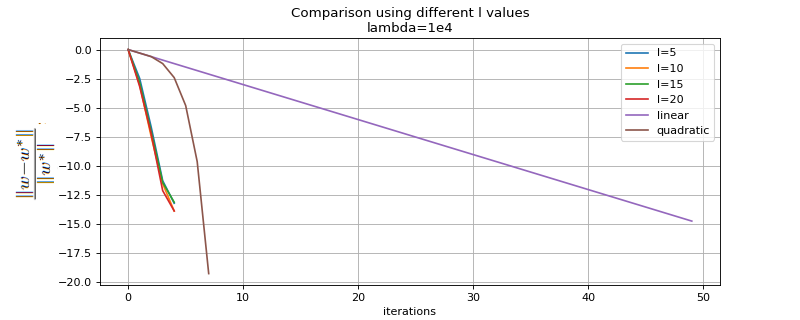
\includegraphics[width=0.8\linewidth]{images/lbfgs/lambda1e4.png}} \\
    \subfloat[Without the convergence rates]{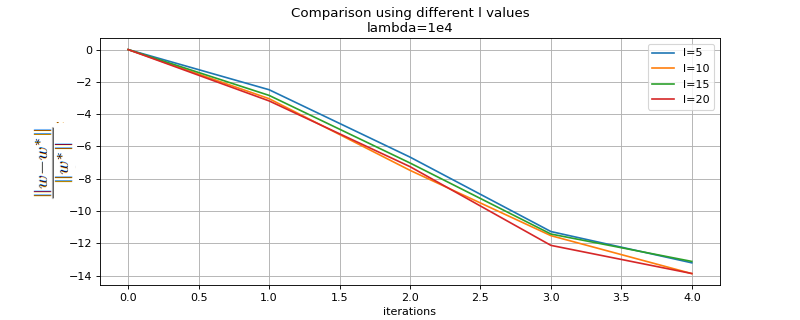
\includegraphics[width=0.8\linewidth]{images/lbfgs/lambda_wout_1e4.png}}
    \caption{Convergence plot with $\lambda=1e4$ at varying values of $l$}
    \label{fig:lbfgs_1e4_l}
\end{figure}

\begin{figure}[H]
    \centering
    \subfloat[Considering the convergence rates]{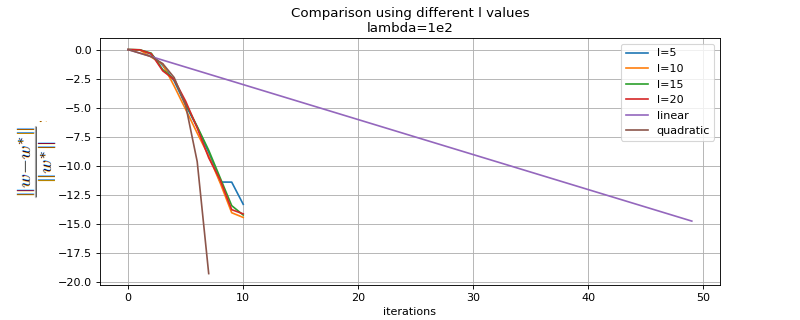
\includegraphics[width=0.8\linewidth]{images/lbfgs/lambda1e2.png}} \\
    \subfloat[Without the convergence rates]{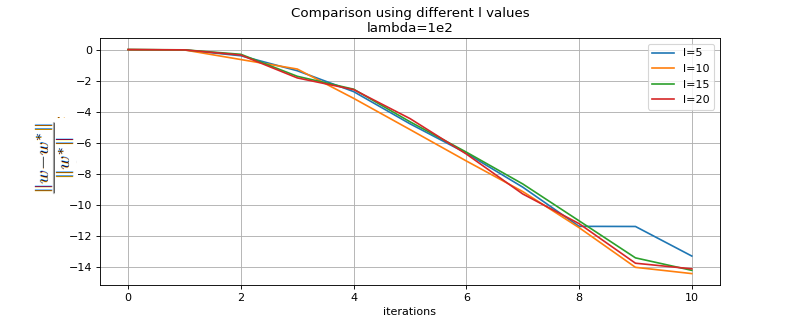
\includegraphics[width=0.8\linewidth]{images/lbfgs/lambda_wout_1e2.png}}
    \caption{Convergence plot with $\lambda=1e2$ at varying values of $l$}
    \label{fig:lbfgs_1e2_l}
\end{figure}


\begin{figure}[H]
    \centering
    \subfloat[Considering the convergence rates]{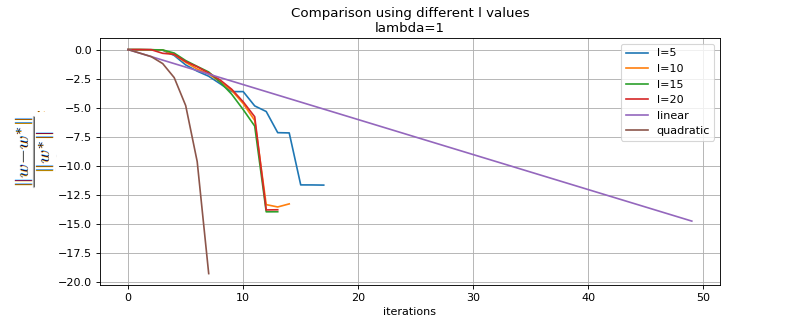
\includegraphics[width=0.8\linewidth]{images/lbfgs/lambda1.png}} \\
    \subfloat[Without the convergence rates]{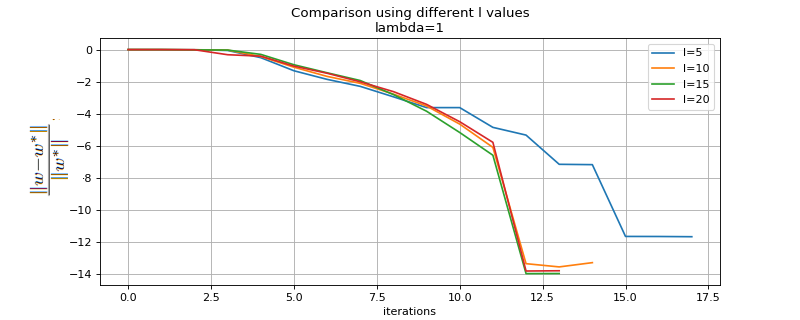
\includegraphics[width=0.8\linewidth]{images/lbfgs/lambda_wout_1.png}}
    \caption{Convergence plot with $\lambda=1$ at varying values of $l$}
    \label{fig:lbfgs_1_l}
\end{figure}

\begin{figure}[H]
    \centering
    \subfloat[Considering the convergence rates]{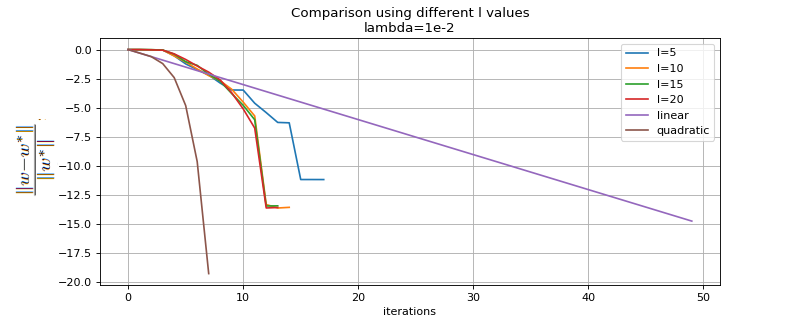
\includegraphics[width=0.8\linewidth]{images/lbfgs/lambda1e-2.png}} \\
    \subfloat[Without the convergence rates]{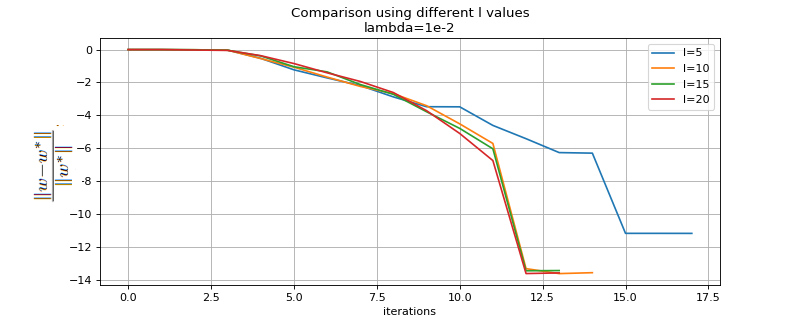
\includegraphics[width=0.8\linewidth]{images/lbfgs/lambda_wout_1e-2.png}}
    \caption{Convergence plot with $\lambda=1e-2$ at varying values of $l$}
    \label{fig:lbfgs_1e-2_l}
\end{figure}

\begin{figure}[H]
    \centering
    \subfloat[Considering the convergence rates]{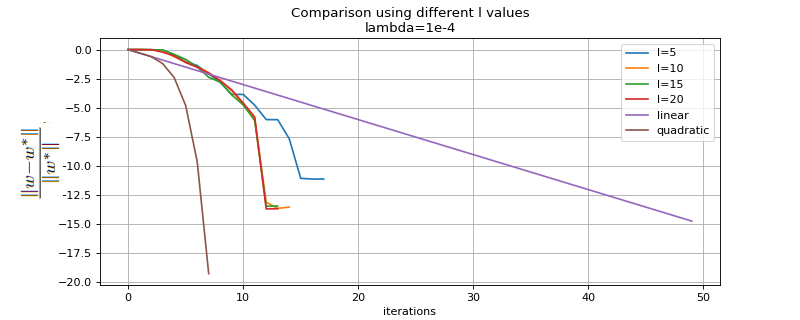
\includegraphics[width=0.8\linewidth]{images/lbfgs/lambda1e-4.png}} \\
    \subfloat[Without the convergence rates]{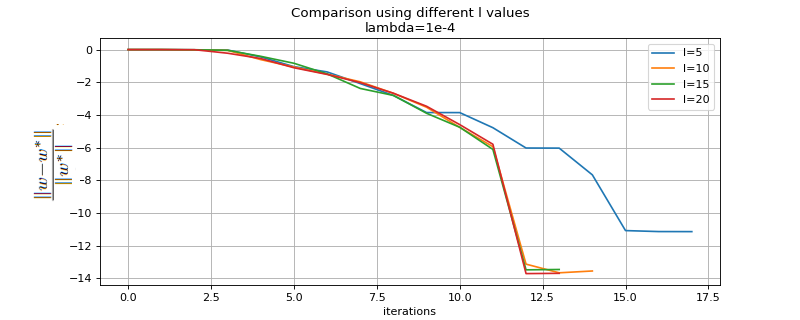
\includegraphics[width=0.8\linewidth]{images/lbfgs/lambda_wout_1e-4.png}}
    \caption{Convergence plot with $\lambda=1e-4$ at varying values of $l$}
    \label{fig:lbfgs_1e-4_l}
\end{figure}
